\chapter{TESTES} % (fold)
\label{cha:testes} % (fold)

\section{Descrição do Experimento}
\label{cha:descricao_do_experimento}

 Será feito um experimento para teste do Sistema de Recomendação de Produtos Dionisio.

 Dionisio é um Sistema que armazena informações sobre produtos e pessoas. As pessoas podem formar uma rede social de amigos e avaliar os produtos, fazendo recomendações para outras pessoas conhecidas ou desconhecidas. A partir das avaliações das pessoas e das relações sociais, o sistema gera listas de recomendações de produtos com o objetivo de ajudar as pessoas a encontrar produtos que elas ainda não conhecem mas possuem grande probabilidade de gostar.

 O experimento consistirá de um período de uso do sistema por grupos de pessoas. Serão 12 grupos com 5 pessoas cada um. Os grupos serão formados da seguinte forma:

\begin{itemize}
	\item Inicialmente serão convidadas 12 pessoas de diferentes faixas etárias.
	\item Será passado um endereço de internet (URL) para cada uma das pessoas se cadastrar no sistema
	\item Será pedido a cada uma dessas pessoas que convide mais 4 amigos ou conhecidos, usando uma ferramenta do próprio sistema, para completar um grupo de 5 pessoas.
\end{itemize}

 O cadastro no sistema consiste de um série de formulários que visam extrair informações demográficas e pessoais. Serão pedidas as seguintes informações:
 
\begin{itemize}
	\item Nome
	\item Sexo (masculino ou feminino)
	\item Data de nascimento
	\item Escolaridade
	\item Foto
\end{itemize}

 Será pedido também que elas avaliem em uma escala de 1 a 10, quais são os produtos que elas possuem o maior interesse para obter recomendações, como:

\begin{itemize}
	\item Roupas
	\item Músicas
	\item Filmes
	\item Eletrônicos
	\item Livros
\end{itemize}

	Depois do cadastro dessas informações iniciais será pedido que cada pessoe avalie as outras pessoas de seu grupo, fornecendo as seguintes informações sobre a outra pessoa:

\begin{itemize}
	\item O quanto ela conhece a outra pessoa. As opções são:
	\subitem Não conhece
  \subitem Conhece pouco
  \subitem Conhece bastante
  \subitem Melhor amiga
  \item O quanto ela confia na outra pessoa para a recomendação de produtos em geral:
  \subitem Não confia
	\subitem Confia um pouco
  \subitem Confia muito
  \subitem Confia completamente
\end{itemize}

 Após o levantamento dessas informações será pedido que cada usuário avalie uma série de produtos aleatórios. Cada produto será apresentado através de uma foto e uma descrição. Será pedido que o usuário escolha em uma escala de 1 a 5 o quanto ele gosta daquele produto caso ele o conheça. Se o usuário não conhecer o produto ele deverá escolher a opção "não conheço".

 Feita essa avaliação, começará o uso pleno do sistema pelo usuário. Dentro do sistema as pessoas terão as seguintes opções:
\begin{enumerate}
	\item Ver listas de recomendações
	\item Procurar por produtos
	\item Fazer uma recomendação
	\item Ver lista de pessoas
\end{enumerate}

 Ao acionar a primeira opção será mostrado ao usuário uma série de diferentes listagens de produtos recomendados. Para cada produto recomendado, o usuário terá a opção de avaliar:

\begin{itemize}
	\item O quanto ele gostou daquela recomendação, em uma escala de 1 a 5.
	\item Opcionalmente, o quanto ele gosta daquele produto.
\end{itemize}

 Uma destas listagens será composta pelas recomendações feitas por outras pessoas. Neste caso também será mostrado além do produto recomendado, quem fez a recomendação e uma justificativa do recomendado para aquela recomendação.

 Ao acionar a segunda opção, o usuário poderá ver os diferentes produtos cadastrados no sistema, podendo filtrá-los através de diferentes critérios. Haverá também uma listagem ordenada dos produtos mais bem avaliados nas diferentes categorias de produtos.

 Ao acionar a terceira opção, o usuário poderá fazer uma busca de um produto para recomendar a uma ou mais pessoas cadastradas no sistema. A recomendação consistirá de um produto e de uma justificativa do porquê daquele produto estar sendo recomendado.

 Ao acionar a quarta opção o usuário poderá ver a lista das pessoas conhecidas ou desconhecidas. Inicialmente apenas as pessoas de seu grupo estarão na lista de conhecidos. Mas ele poderá escolher uma outra pessoa para entrar em sua lista de conhecidos fazendo um pedido de amizade.

 A lista de pessoas possue um atalho para o perfil de cada usuário. Este perfil é composto do nome, idade, sexo, foto da pessoa e uma lista dos produtos avaliados por essa pessoa.

 O sistema estará disponível por um período de 1 mês, sendo que ao final o mesmo será desativado e sua base de dados será analisada de forma anônima para se medir qual foi a eficácia das recomendações feitas pelo sistema e entre os usuários.

\section{Protótipo}
\label{cha:prototipo}

 Um protótipo do sistema foi desenvolvido para que se pudesse ter noção da usabilidade e do funcionamento do sistema de recomendação. Inicialmente as recomendações são realizadas sem levar em conta os dados de confiança e reputação entre usuários, além de solicitar apenas o nome e e-mail da pessoa. A Figura~\ref{fig:tela_inicial_prototipo} mostra a página inicial do protótipo, contendo a listagem dos primeiros produtos presentes na base de dados e a opção do usuário fazer o \textit{login} no sistema.
 
\begin{figure}
  \centering
  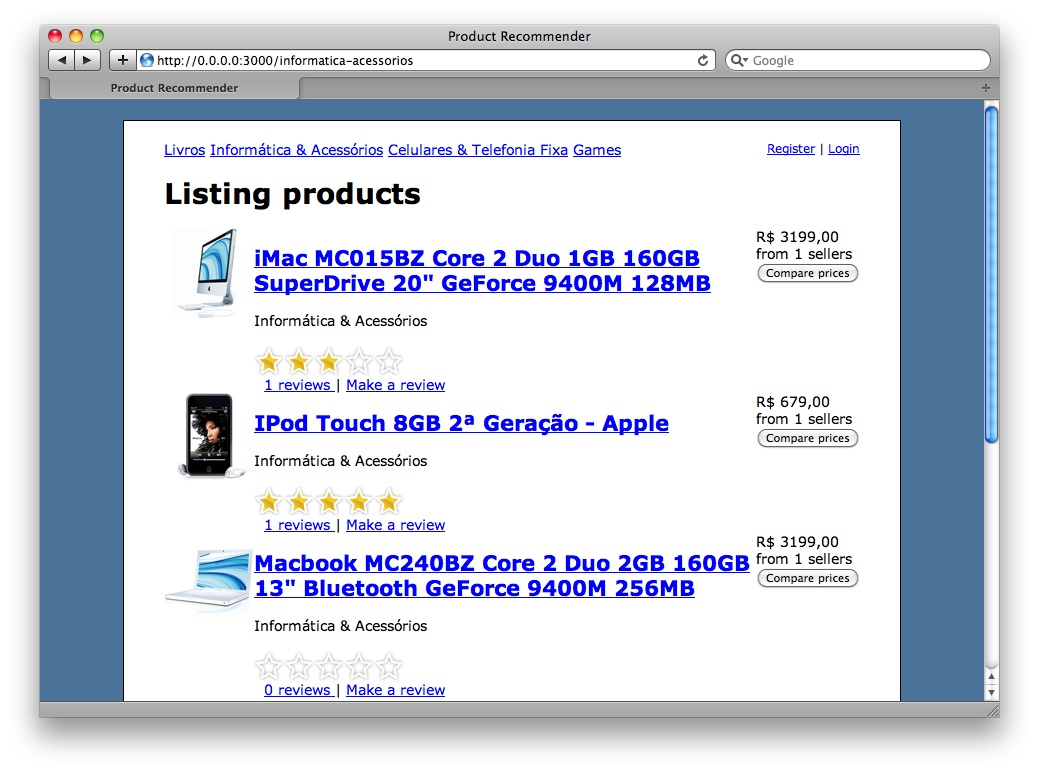
\includegraphics[width=\textwidth]{imagens/Tela_Inicial_Prototipo}
  \caption{\it Tela inicial do protótipo}
  \label{fig:tela_inicial_prototipo}
\end{figure}

 A tela de \textit{login} solicita apenas o nome de usuário e senha, conforme ilustrado na Figura~\ref{fig:tela_login_prototipo}. Após a validação dos dados, o sistema retorna para a tela inicial para que o usuário possa detalhar um produto de seu interesse. Ao escolher um produto, o sistema abre os seus detalhes incluindo nome, foto e descrição completa, como mostra a Figura~\ref{fig:detalhe_produto_prototipo}.

\begin{figure}
  \centering
  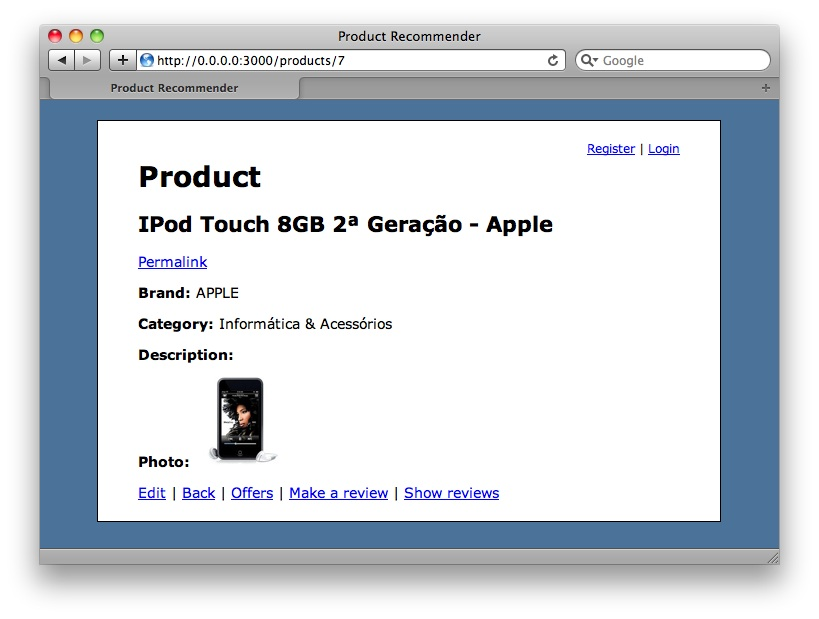
\includegraphics[width=\textwidth]{imagens/Detalhe_Produto_Prototipo}
  \caption{\it Detalhe do produto}
  \label{fig:detalhe_produto_prototipo}
\end{figure}